\graphicspath{{img/ch6}}

\section{Potential for Permanent Human Presence}

\subsubsection{Radiation and Micrometeoroid Shielding}

Lunar pits offer significant protection against radiation and micrometeoroid impacts, which are two of the most hazardous environmental conditions on the Moon's surface. Without a magnetic field or atmosphere, the Moon is exposed to intense solar and galactic cosmic radiation, as well as a constant flux of micrometeoroid impacts. However, the overlying material within pits acts as a natural barrier, significantly attenuating these threats. 

Studies indicate that radiation levels within pits are drastically reduced compared to surface conditions, providing a safer environment for equipment and potential human habitats \cite{thermal-lunar-pits, newer-thermal}. This is particularly relevant for the protection of astronauts from galactic cosmic radiation (GCRs) and solar particle events (SPEs), which can cause acute and long-term health effects. Measurements and models of the radiation environment inside lunar pits suggest that the radiation dose experienced within pits is comparable to that inside lava tubes, where the thickness of the overlying roof (often exceeding 10 m) is sufficient to block high-energy cosmic particles \cite{bases-feng}.

Micrometeoroid shielding is another major advantage of lunar pits. The steep vertical walls and overhanging entrances intercept incoming micrometeoroids, protecting the base of the pit from impacts. This natural shielding effect extends the operational lifespan of surface-deployed equipment and reduces the risk of structural damage to human habitats. For long-term human missions, such protection is critical for reducing exposure to cumulative radiation doses and preventing punctures in habitat pressure vessels. Lava tubes have demonstrated natural resistance to impact damage due to their **robust roof thickness and basaltic composition**, as confirmed by **GRAIL gravity data** and **Mini-RF radar observations** \cite{bases-feng, Carrer2024}.

\subsubsection{Resource Potential}

Lunar pits provide a valuable opportunity for **in-situ resource utilization (ISRU)**, particularly with respect to the extraction and storage of water ice and volatiles. In regions near the lunar poles or areas where parts of the pit floor are permanently shadowed, it is possible that water ice may be present. These volatiles are critical for sustainable human exploration because water can be split into hydrogen and oxygen, serving as fuel for rocket propulsion, while oxygen can be used directly for life support systems \cite{jsanders-isru}.

The geometry of pits may promote volatile trapping, especially if the surrounding exterior topography casts shadows onto the pit floor. Unlike impact craters, the **overhangs of pits limit the amount of reflected infrared radiation** entering the structure, reducing thermal fluctuations. This effect could provide favorable conditions for water ice stability, although multiple scattering of infrared radiation within the pit may still elevate interior temperatures beyond optimal cold-trapping conditions \cite{newer-thermal}.

Another promising opportunity is the use of pits for **resource storage and ISRU operations**. The stable thermal environment of pits can support the storage of extracted volatiles, fuel, and other materials. Unlike surface storage facilities, which must endure extreme thermal cycles, ISRU stations within pits would be shielded from both temperature extremes and impact hazards. This stable environment reduces the maintenance requirements for ISRU machinery and extends the operational lifespan of oxygen extraction systems, regolith processing units, and **water-ice harvesting systems** \cite{jsanders-isru, thermal-lunar-pits}.

\subsection{Lunar Base Construction}

Lunar pits are prime candidates for the construction of future **lunar bases** due to their natural shielding, structural stability, and potential access to subsurface cavities. Establishing a base within a pit would significantly reduce the amount of infrastructure required to protect astronauts and equipment from radiation, micrometeoroids, and temperature extremes. Studies of potential sites, such as the **Mare Tranquillitatis pit** and the **Marius Hills pits**, suggest that their structural stability and accessibility make them ideal locations for long-term human presence on the Moon \cite{new-wagner, Carrer2024}.


\begin{figure}[H]
    \centering
    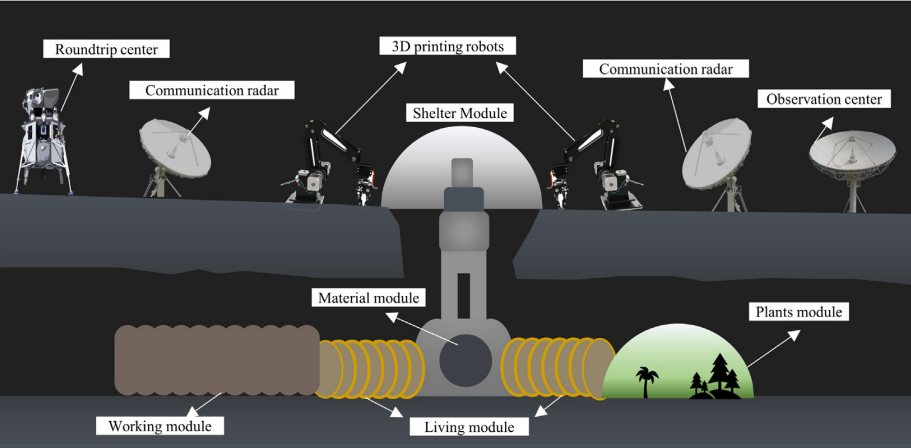
\includegraphics[width=0.75\linewidth]{simple-base-schema.png}
    \caption{Conceptual design of a lunar base within a pit. The natural overhangs provide protection against radiation and micrometeoroid impacts, while modular inflatable habitats offer pressurized living space. Adapted from \cite{bases-feng}.}
    \label{fig:lunar-pit-habitat-concept}
\end{figure}


\subsubsection{Architectural Concepts for Lunar Bases}

Current proposals for lunar base designs include **modular pressurized habitats** or **inflatable living spaces** deployed inside pits. The natural rock overhangs provide primary shielding, while inflatable habitats or regolith-filled barriers offer secondary protection. 

Another proposed method involves **structural reinforcement of pit walls** using autonomous construction rovers. The rovers would deposit layers of regolith over the habitat to increase shielding. Modular components could also be anchored to the walls of the pit using drill-based attachments or hooks. This approach avoids the need to import heavy building materials from Earth and allows for lightweight construction techniques.

\subsubsection{Exploration and Construction Strategies}

Exploration missions will likely precede human base construction. These initial missions would rely on **tethered climbers, robotic hoppers, or drones** to navigate the steep vertical walls of pits. Robots like **NASA's Daedalus concept** or the ESA **Daedalus rover** are designed to rappel down pit walls and map the internal structure of voids beneath the surface. By mapping potential entry points into subsurface voids, such missions will identify sites for future human exploration and establish the geological integrity of the location \cite{Carrer2024}.

Once a site is confirmed as stable, human missions could begin **surface-based construction** by sealing off portions of pits to create enclosed, pressurized living spaces. The strong basaltic rock found at sites like Marius Hills and Mare Tranquillitatis is a favorable construction material due to its strength and durability \cite{new-wagner}. Human crews may use **ISRU technology** to convert regolith into building materials, further supporting the development of long-term habitats.


\subsection{Advanced ISRU Capabilities}

Lunar pits offer strategic advantages for the establishment of \textbf{advanced ISRU (In-Situ Resource Utilization) stations}. The naturally stable environment of pits reduces the operational constraints on ISRU equipment, such as temperature fluctuations, solar radiation exposure, and impact hazards. This section focuses on the potential for water harvesting, oxygen production, and regolith processing within pits.


\subsubsection{Water Ice Extraction and Volatile Harvesting}

Regions within pits that experience **permanent shadowing** may accumulate water ice and volatiles. Unlike surface-based extraction, pit-based harvesting is more thermally stable and avoids the risks of solar variability. Water ice could be extracted and converted into hydrogen and oxygen via **electrolysis systems**. These gases serve as propellants and can also support life support systems \cite{jsanders-isru}.



\subsubsection{Oxygen Production from Regolith}

Oxygen can be extracted from lunar regolith using \textbf{molten regolith electrolysis} or chemical reduction of ilmenite. Establishing oxygen production stations within pits allows the machinery to operate in stable conditions, free from solar heating and rapid cooling cycles. This reduces maintenance and operational failures, making it feasible to maintain continuous production. According to \textbf{NASA's ISRU roadmap}, \textbf{Artemis missions} will aim to establish ISRU oxygen production on the Moon by the 2030s \cite{jsanders-isru}.

\subsubsection{Regolith Processing and Additive Manufacturing}

Another application of ISRU is the \textbf{processing of regolith into construction materials}. Lunar regolith can be used to produce \textbf{regolith bricks} via sintering or 3D printing. By placing production stations within pits, engineers can take advantage of thermal stability, ensuring consistent sintering conditions for manufacturing. 3D printing technologies could enable on-site production of habitat modules, walkways, and storage units, significantly reducing the mass of construction materials needed from Earth \cite{bases-feng, jsanders-isru}.